\documentclass[12pt, openany]{report}

\usepackage[english]{babel}
\usepackage{setspace}
\usepackage{parskip}
\usepackage[utf8]{inputenc}
\usepackage{hyperref}
\usepackage[pdftex]{graphicx}
\usepackage[toc,page]{appendix}
\setlength{\parindent}{15pt}
\renewcommand{\thesection}{\arabic{section}}
\makeatletter\@openrightfalse\makeatother

\setstretch{1.3}

\begin{document}
\begin{titlepage}
\author{
        Braulio Grana Gutiérrez \\
        \href{mailto:bgg@kth.se}
        {bgg@kth.se}
        \and
        Adrián Ramírez del Río \\
        \href{adrianra@kth.se}
        {adrianra@kth.se} }

\title{{\Huge Analysis of crime in London}}
\maketitle
\end{titlepage}

\pagenumbering{roman}
\tableofcontents
\listoffigures

\begin{abstract}

Nowadays, cities are producing a huge amount of data from several sources: traffic, air pollution, hospitals and energy among others. In the biggest and more advanced cities this data is even publicly available via APIs (Application Programming Interfaces). We believe that all those data can be put to good use to analyze the great problems that european cities are facing nowadays.

With that objective we have decided to analyze the problem of criminality as it is one of the most common problems in big cities and one of the most impactful in citizens' lives. In order to do that we are gathering data from official sources in London to identify correlations and patterns that can help us find the factors that are most relevant for each kind of crime. Notice that correlation does not equal causality so we are not claiming the factors we find to be causes of high crime rates, but if we were to find certain patterns of correlations repeating over the years of data it could give hints about where should the legislators look for the source of the problems.

Lastly, we are doing this research with the hope that it will become a useful source of information for politicians when trying to know where to put their efforts in order to reduce the problems of criminality in big cities. As we hope for the information we generate to actually be used, we are being extremely careful to not draw conclusions that may lead to generate hatred against certain groups of people living in the cities.

\end{abstract}

\pagenumbering{arabic}

\section{Introduction}

Currently there is a huge demand for extracting useful information generated by modern societies both on the internet and in the physical world. This demand does not come from the private sector only as more and more government institutions are starting their own Data Science projects to take advantage of the tremendous amount of data they already manage.

Among these government institutions, city halls are among the most eager as they manage large amounts of data, especially in big capital cities such as Stockholm, London or Berlin. Cities nowadays gather data  through millions of monitoring devices spread across their territory. The data collected ranges from environmental, such as air or water pollution, to more day-to-day affairs like unemployment rates, birth rates or energy consumption. These data are publicly available for many european cities coming from official government sources, although some of them still do not have it available through a digital access point such as an API.

Using all these data, we plan to study the relevant factors for criminality in London, as it has a huge database of datasets from a large range of years. Having such an incredible amount of data we will be able to find relevant factors for high crime rates and, depending on the granularity of the city's data we could relate these factors to specific types of crimes.

We do not expect to come to direct cause-effect conclusions as finding correlations is not the same as finding causes, but if we find repeating patterns associated to high criminality rates, the information could be of great use for future legislators looking to decrease this problem.

\section{Theoretical framework}

It has been hard to find literature related to the proposed topic, which make us think it is interesting and effort should be put in order to study it further. The majority of the found bibliography focus either on predicting crime data by means of machine \cite{mcclendon15} and statistical learning \cite{berk09} or on finding specific crime patterns that can help crime analysts to identify series of related crimes \cite{wang13}.

It comes to our minds that there is a lack in the understanding of why crime is present and what factors should be looked at in order to understand and prevent it. Thus our focus would be not only to analyze the data with statistical techniques in order to find correlations, but also to use the methods for crime prediction shown in previous work [1, 2] (or some similar predictive methods) and further analyze the predictive models in order to find important variables that these models focus on whilst performing the predictive task.

\section{Research questions}

For our hypothesis, we will investigate official thresholds for different criminality types above which an area is considered to have “high criminality”. Using this we will perform a classification analysis to find out which boroughs of London have had the highest criminality and in which years.

Ultimately, this will allow us to identify the relevant factors of high criminality for different types of crimes in London between the years 2005 and 2014.

\section{Method}

We will try to follow the CRISP-DM methodology [4] which is specifically designed for data mining processes in the industrial environment. In our special case, where we are not interested in a commercial advantage of the obtained results (we are only performing a research study) some of the phases described will be accordingly modified. The “Business Understanding” phase will turn into the understanding of the theoretical framework and literature. For the “Evaluation” phase, we will rather draw conclusions from the results, and finally, no “Deployment” phase will be necessary.

Note this is an iterative methodology, and as so we shall make several passes over the data and the generated results.

\section{Results and Analysis}


\subsection{Data gathering and preprocessing}

We have gathered data from official sources (APIs) from London open data portal. We have selected and cleaned the following datasets between 2005 and 2014 as part of our analysis:

\begin{itemize}

\item Employment/Unemployment rates
\item Births by birthplaces of mother
\item Births and fertility rates
\item Population estimates
\item Average income of taxpayers
\item Number and density of dwellings
\item Carbon emissions
\item Business demographics
\item Crime data
\item Job seeker allowances

\end{itemize}

The dataset were initially extremely different between each other in terms of structure, time periods, periodicity and format. We used several Python and Bash scripts to clean and preprocess the dataset to a point where they could be merged together using the python functool library's reduce function. Lastly, we normalized the population data to a per 100k basis since it is the most common measure for crime rates.

%% IMAGE of the final merged dataset
\begin{figure}[h!]
\centering
        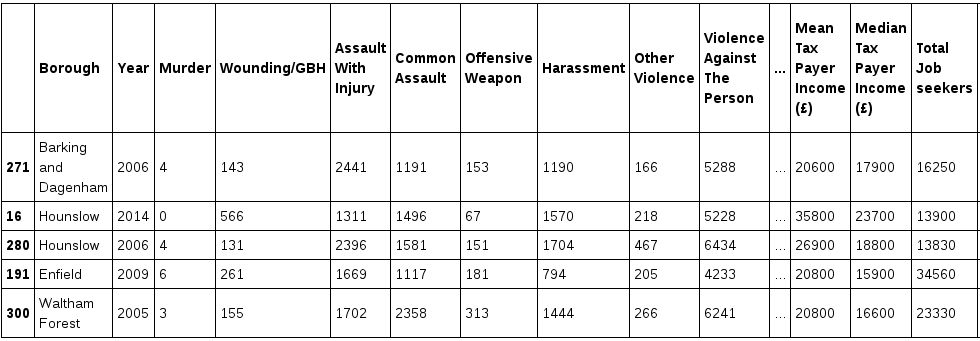
\includegraphics[width=0.8\textwidth]{images/merged_dataset.png}
        \caption{Merged dataset}
\end{figure}

Once we collected, preprocessed, cleaned and merged the data from all the datasets above we proceeded to perform a descriptive analysis of our data to give the reader a better understanding of the dataset’s structure and some variables.

%% PLOT crimes over boroughs
\begin{figure}[h!]
\centering
        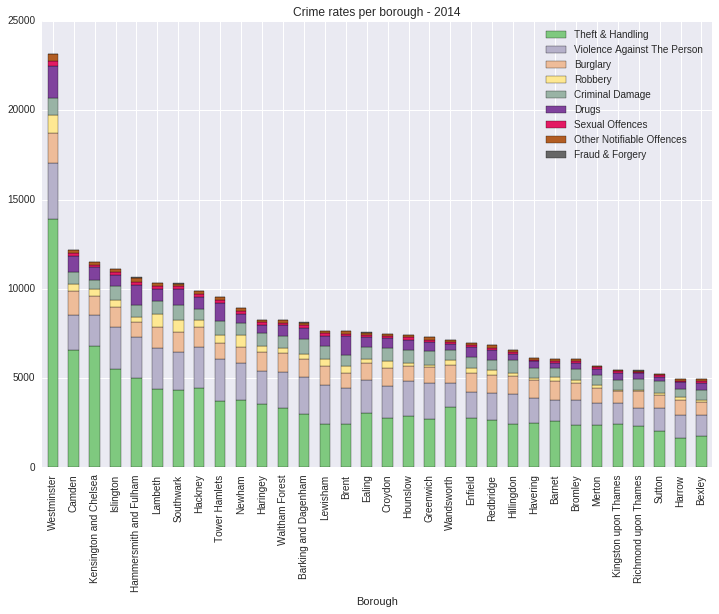
\includegraphics[width=0.8\textwidth]{images/crimes_borough_2014.png}
        \caption{Crime rates over boroughs in 2014}
\end{figure}

The overall structure has a year and a borough per row and then all the different variables that we have gathered, this way we can perform a classification analysis of the city over the course of a decade. We have performed some simple exploratory analysis.

%% PLOT total crime evolution by year
\begin{figure}[h!]
\centering
        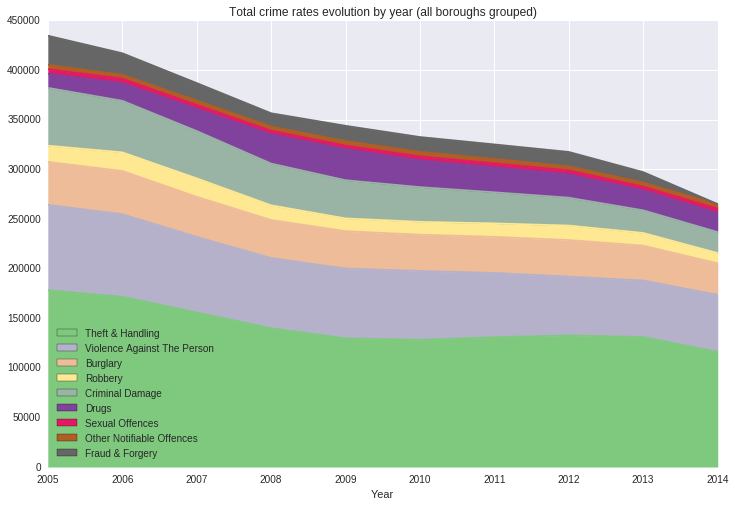
\includegraphics[width=0.8\textwidth]{images/crime_evolution_total.png}
        \caption{Crime evolution per year in all boroughs}
\end{figure}

So, in total, we are dealing with 9 crime categories, 32 subcategories, across 32 boroughs for 10 years in a yearly basis. Therefore, we have 320 observations in our final dataset.

\subsection{Modeling}

For the modeling part we applied the same process to the 9 crime categories:

\begin{enumerate}

\item Categorize observations using a binary categorization divided by a threshold chosen as the overall mean of the 320 observations since we did not find any official threshold values for high crime rates.

%% IMAGE of threshold
\begin{figure}[h!]
\centering
        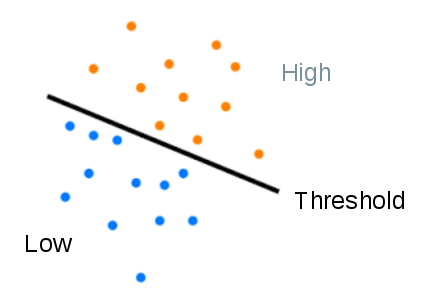
\includegraphics[width=0.8\textwidth]{images/threshold.png}
        \caption{Binary class threshold}
\end{figure}

\item Divide data in train/test: In our case we used a 75\% training and 25\% testing ratio. The sampling was done using a technique called stratified random sampling, that allowed us to get proportional samples from each of the types of crime.

%% IMAGE explaining stratified random sampling
\begin{figure}[h!]
\centering
        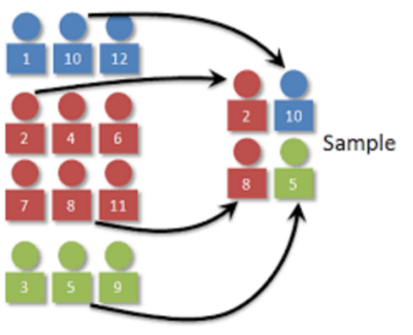
\includegraphics[width=0.8\textwidth]{images/strata_sample.png}
        \caption{Stratified random sampling example}
\end{figure}

\item Train the model using a random forest classifier \cite{breiman01}. For this part we allowed bootstraping and we used all the features (variables) in our dataset. We also weighted observations based on class imbalance.
\item Evaluate the model by trying it against the testing dataset and extracting useful measures like its confusion matrix.

%% Image of confusion matrix
\begin{figure}[h!]
\centering
        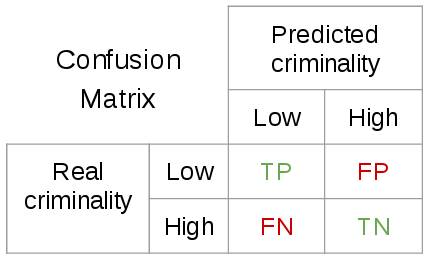
\includegraphics[width=0.8\textwidth]{images/confusion_matrix.png}
        \caption{Confusion matrix}
\end{figure}

\item Retrain the model with the same parameters on the whole dataset as this allows better calculation of feature importance.
\item Compute factor importance using the gini importance measure \cite{breiman84}, which orders factors according to their importance.

\end{enumerate}

Here we show the results obtained for the crime class violence against the person as an example:

%% PLOT violence against the person results
\begin{figure}[h!]
\centering
        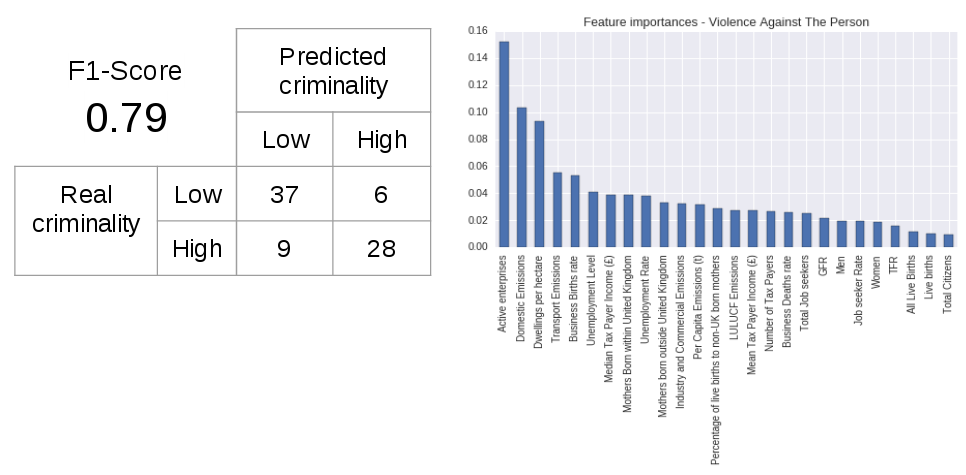
\includegraphics[width=0.8\textwidth]{images/results_violence_person.png}
        \caption{Results for violence against the person}
\end{figure}

For this type of class we can see that Active enterprises, Domestic Emissions and Dwellings per hectare identified as important factors for the classification algorithm.


The complete results for each type of crime can be found in the code. Appendix \ref{appendix:code} has a link to the Github repository containing it.

\section{Discussion}

In this section, we would like to discuss the moral implications of handling data coming from citizens, even when these data are just aggregates they still link to certain groups of people by their ethnicity, nationality, religion, income and many other factors. For this reason we would like to be extremely careful not to draw wrong conclusions that may hurt the image or even the lives of the citizens we are analyzing.

This said, we will not in any case change the results coming from our study to be politically correct with any group. What we will do is guarantee that all our data come from official governmental sources so we can be confident that it has not been contaminated with biases by other interested parties.

\section{Conclusions}

After completing the work we can conclude that, as we had hypothesized, some factors seem to work better in order to explain high criminality rates, and these depend on the type of crime considered.

Also, the factors found aren’t necessarily the cause of the criminality, so expert crime analysts should look into them and try to find why they correlate. Sometimes, the considered factors are not good enough to explain the high crime rates, so the produced models should be evaluated in order to avoid drawing wrong conclusions.

\section{Future work}

As for future work and improvements in the current work, we spotted possibilities:

\begin{itemize}

\item Include more data sources with factors that could be relevant for the analysis.
\item Include more data sources with criminality rates of other areas or even other cities.
\item Further investigate the crime analysis literature to see how criminality rates thresholds are usually applied in order to differentiate high/low criminality areas.
\item Try performing the analysis with more specific types of crime.
\item Tune model's hyperparameters with cross validation.

\end{itemize}

\begin{appendices}
\chapter{Dataset links}
\begin{itemize}
\item \href{https://data.london.gov.uk/dataset/economic-activity-rate-employment-rate-and-unemployment-rate-ethnic-group-national/}{Employment/Unemployment rates}
\item \href{https://data.london.gov.uk/dataset/births-birthplace-mother-borough/}{Births by birthplaces of mother}
\item \href{https://data.london.gov.uk/dataset/births-and-fertility-rates-borough/}{Births and fertility rates}
\item 
\href{https://data.london.gov.uk/dataset/office-national-statistics-ons-population-estimates-borough}{Population estimates}
\item \href{https://data.london.gov.uk/dataset/average-income-tax-payers-borough/}{Average income of taxpayers}
\item \href{https://data.london.gov.uk/dataset/number-and-density-of-dwellings-by-borough/}{Number and density of dwellings}
\item \href{https://data.london.gov.uk/dataset/carbon-dioxide-emissions-borough/}{Carbon emissions}
\item \href{https://data.london.gov.uk/dataset/business-demographics-and-survival-rates-borough/}{Business demographics}
\item \href{http://maps.met.police.uk/tables.htm}{Crime data}
\item \href{https://data.london.gov.uk/dataset/job-seekers-allowance-claimants-borough/}{Job seeker allowances}
\end{itemize}

\chapter{Code}
\label{appendix:code}

Github repository: \url{https://github.com/AdrianRamirezRio/crimeAnalysis}	

\end{appendices}

\begin{thebibliography}{10}

\bibitem{powers11} Powers, D. M. W., “Evaluation: From Precision, Recall and F-Measure to ROC, Informedness, Markedness \& Correlation”. 2011, Journal of Machine Learning Technologies 2: 37-63.

\bibitem{mcclendon15} Lawrence McClendon and Natarajan Meghanathan, “Using Machine Learning Algorithms to Analyze Crime Data”. 2015, Machine Learning and Applications: An International Journal (MLAIJ) Vol.2, No.1.

\bibitem{berk09} Berk,  R.,  Sherman,  L.,  Barnes,  G.,  Kurtz,  E.,  Ahlman,  L., “Forecasting  murder within  a  population  of  probationers  and parolees: a high stakes application of statistical learning”. 2009, Journal of the Royal Statistical Society: Series A (Statistics in Society) 172: 191-211.

\bibitem{wang13} Wang, T., Rudin C., Wagner D., Sevieri R., “Learning to Detect Patterns of Crime”. 2013, Machine Learning and Knowledge Discovery in Databases. ECML PKDD 2013. Lecture Notes in Computer Science, vol 8190.

\bibitem{shearer00} Shearer, C., “The CRISP-DM model: the new blueprint for data mining”. 2000, Journal of data warehousing, 5(4), 13-22.

\bibitem{breiman01} Breiman, L., “Random forests”. 2001, Machine learning, 45(1):5–32.

\bibitem{breiman84} Breiman, L., Freidman, J.H., Olsen, R.A., Stone, C.G., “Classification and regression trees”. 1984, Belmont, California: Wadsworth International Group.

\end{thebibliography}

\end{document}
